\chapter{Rezultati}
Dana su nam 3 genoma za testiranje:
\begin{enumerate}
\item EColi - sintetski podaci (3 contig-a)
\item CJejuni - stvarni podaci (6 contig-a)
\item BGrahamii - stvarni podaci (6 contiga-a)
\end{enumerate}
\section{EColi}
Kod EColi smo uspjeli ostvariti skoro savršenu pododarnost kao što vidimo na slici \ref{fig:ecoli}.

\begin{figure}[H]
    \centering
    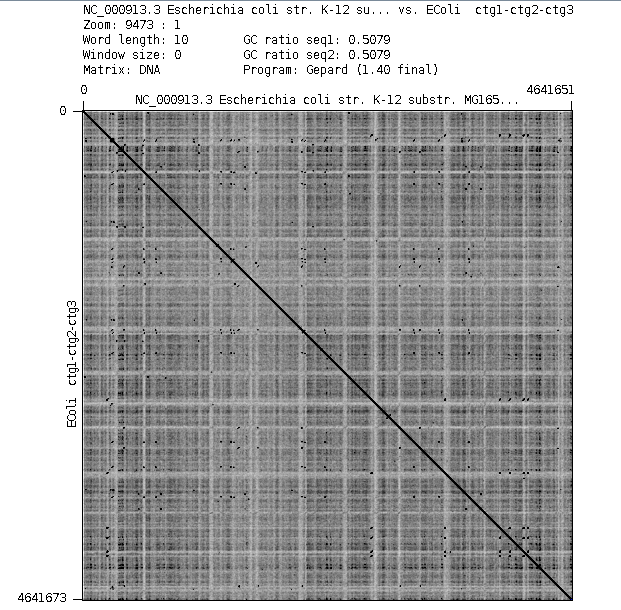
\includegraphics[scale=0.45]{img/EColi.png}
    \caption{EColi - rezultati s Geparda}
    \label{fig:ecoli}
\end{figure}

Duljina referentne sekvence je 4,641,651, a naše 4,641,673 baza. GC omjer je za obje sekvence jednak. Naravno da i podudarnost nismo dobili na bazu, ali smo uspjeli dobiti jednu konzistentnu sekvencu. Količina vremena koja je potrebna da se sastavi genom je u prosjeku 10 sekundi, a zauzima otprilike 50 MiB memorije.

\section{CJejuni}
Kod CJejuni nismo uspjeli dobiti sekvencu koja je u potpunosti u skladu s referencom. U nastavku slijedi nekoliko vrijednih pokušaja. Za procesiranje ovih podataka je potrebna 1 minuta i 200 MiB memorije. 


Najdulja sekvenca koju smo dobili je Ctg2-Ctg4-Ctg5-ctg1-Ctg3-Ctg0. Iako smo povezali sve contige u jednu sekvencu, nisu povezani potpuno točno. Uspjeli smo puno bolje naći manje dijelove od par sekvenca i povezati ih kao što vidimo na narednim slikama.


\begin{figure}[H]
    \centering
    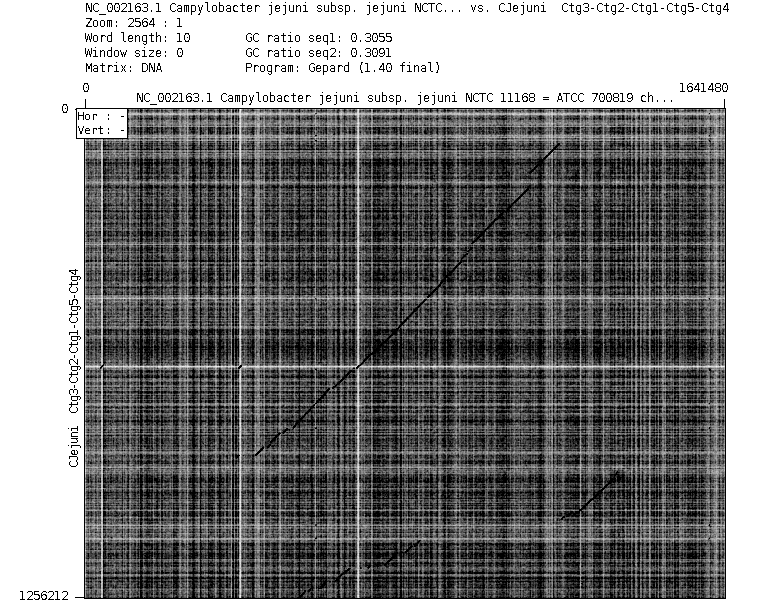
\includegraphics[scale=0.5]{img/Grah8.png}
    \caption{CJejuni - rezultati s Geparda 1}
    \label{fig:cjejuni1}
\end{figure}


\begin{figure}[H]
    \centering
    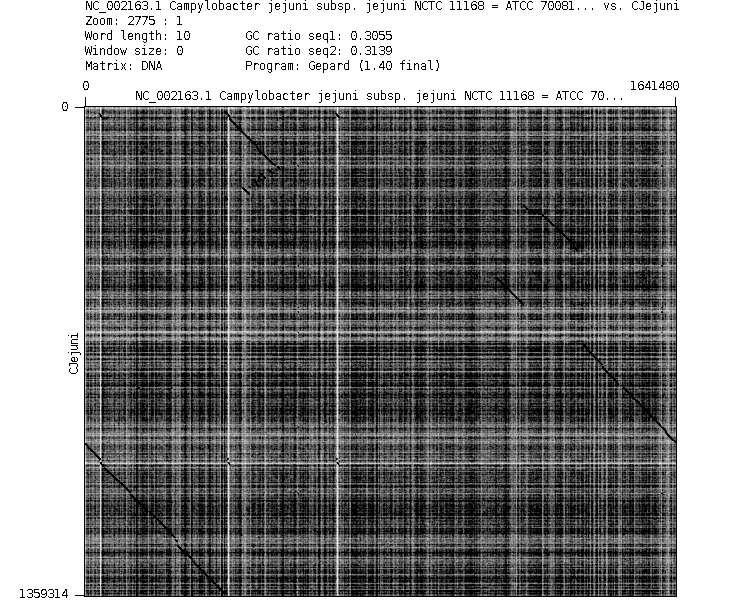
\includegraphics[scale=0.5]{img/Grah10.png}
    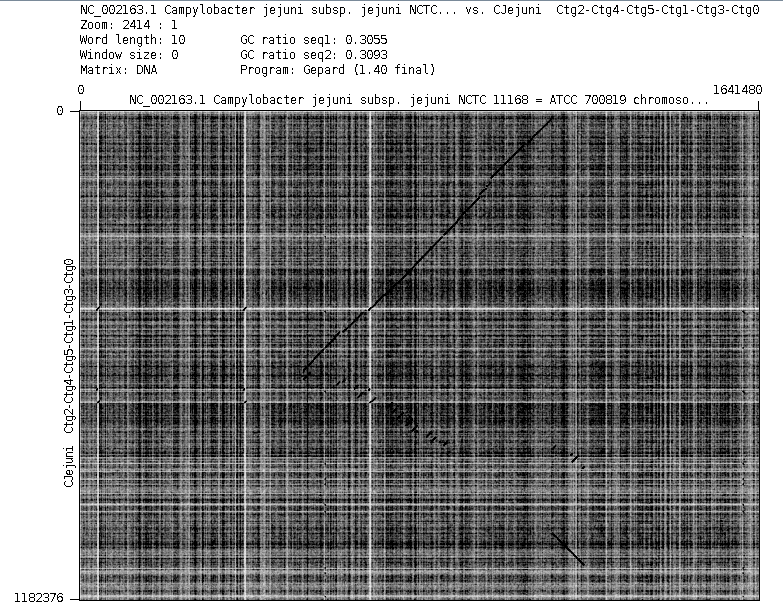
\includegraphics[scale=0.5]{img/Grah1.png}
    \caption{CJejuni - rezultati s Geparda 2}
    \label{fig:cjejuni2}
\end{figure}

\begin{figure}[H]
    \centering
    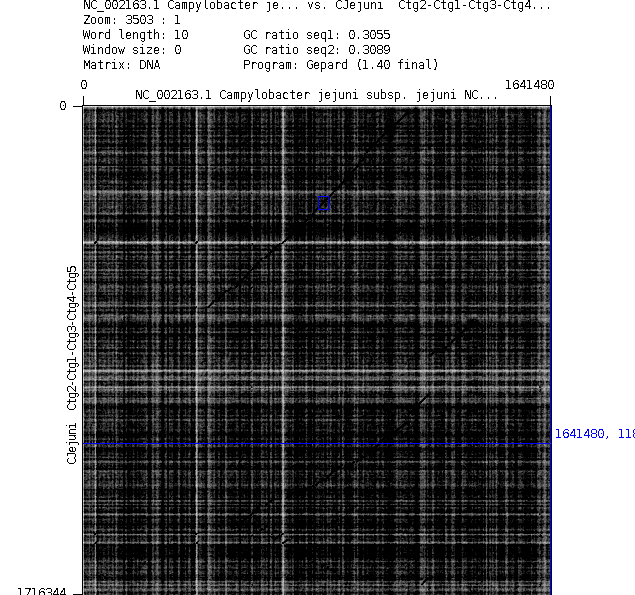
\includegraphics[scale=0.7]{img/Grah2.png}
    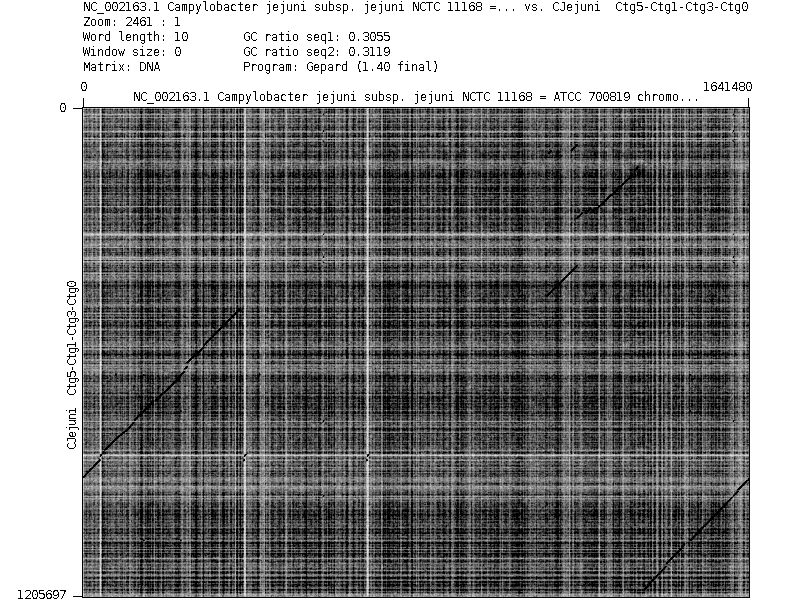
\includegraphics[scale=0.5]{img/Grah3.png}
    \caption{CJejuni - rezultati s Geparda 3}
    \label{fig:cjejuni3}
\end{figure}

\begin{figure}[H]
    \centering
    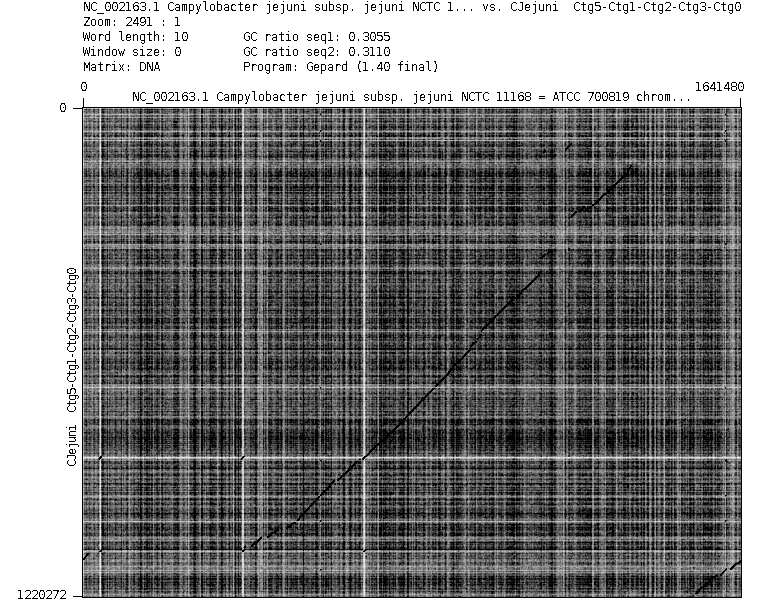
\includegraphics[scale=0.5]{img/Grah4.png}
    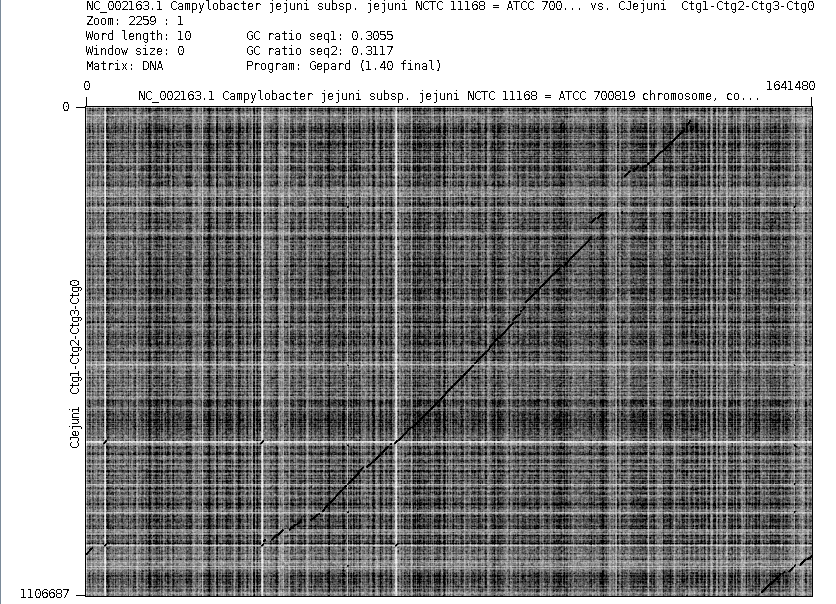
\includegraphics[scale=0.5]{img/Grah5.png}
    \caption{CJejuni - rezultati s Geparda 4}
    \label{fig:cjejuni4}
\end{figure}

\begin{figure}[H]
    \centering
    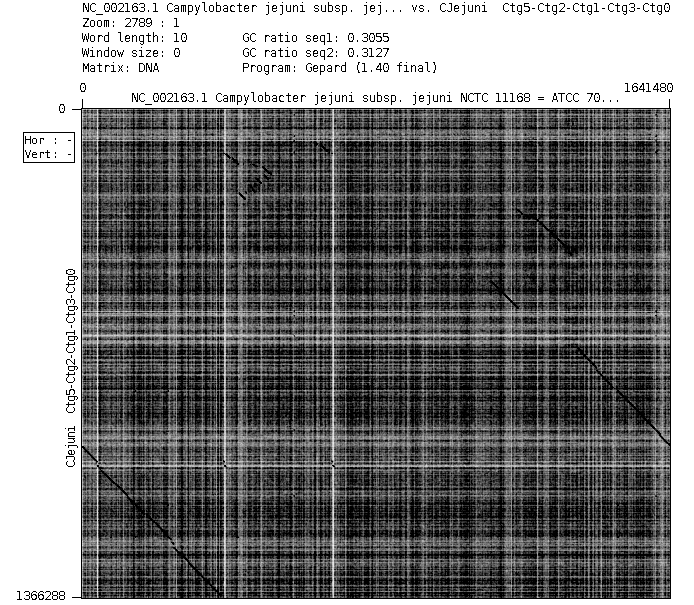
\includegraphics[scale=0.5]{img/Grah9.png}    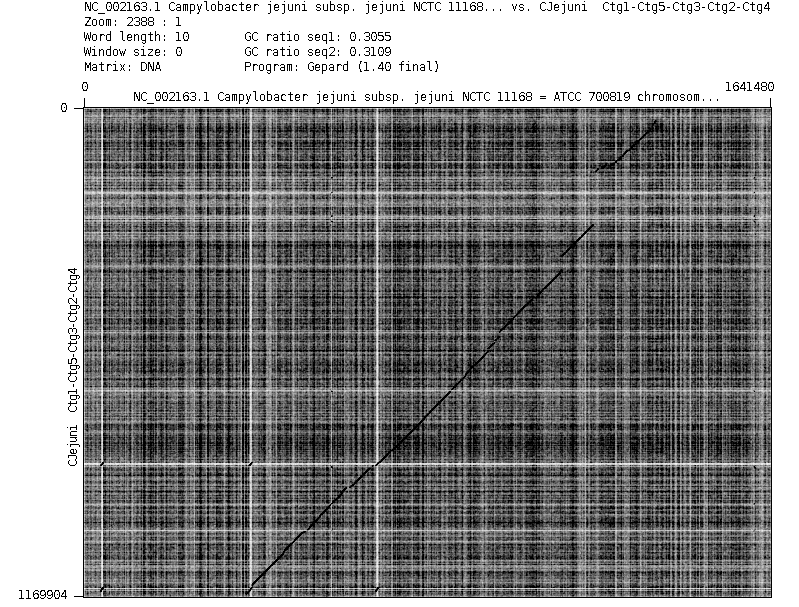
\includegraphics[scale=0.5]{img/Grah6.png}
    \caption{CJejuni - rezultati s Geparda 5}
    \label{fig:cjejuni5}
\end{figure}

\section{BGrahamii}
Rezultati kod BGrahamii genoma isto se ne poklapaju u potpunosti s referentnom sekvencom. Za procesiranje ovih podataka je potrebno 3-10 minuta i 2 GiB memorije (ovisno o parametrima programa). Sastavljene sekvence su vidljive na slikama u nastavku.

\begin{figure}[H]
    \centering
    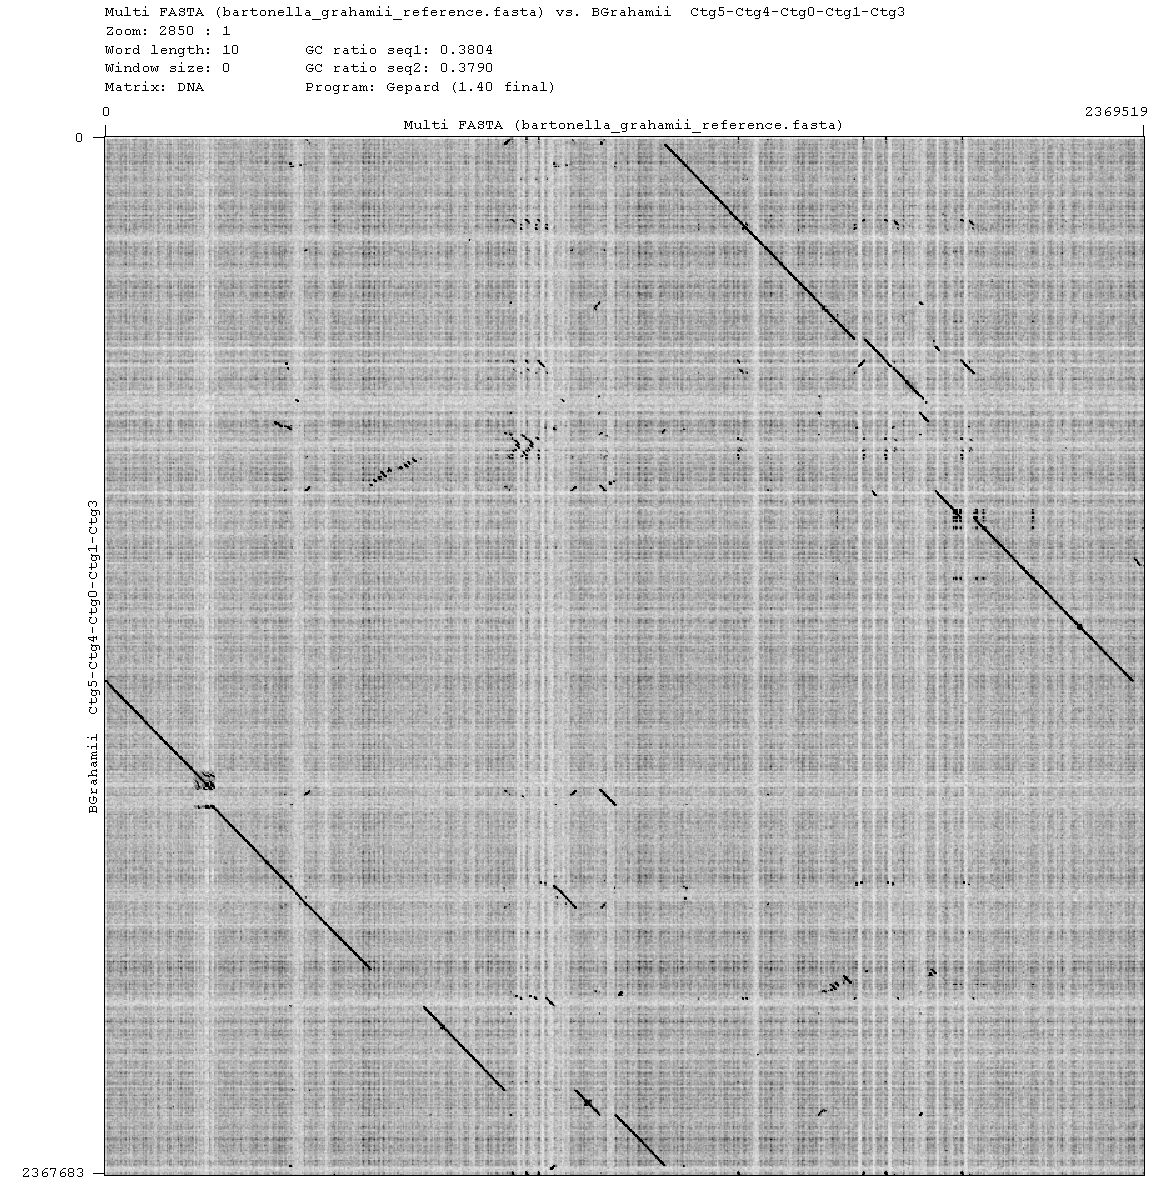
\includegraphics[scale=0.5]{img/graph11.png}
    \caption{BGrahamii - rezultati s Geparda 1}
    \label{fig:bgrahamii1}
\end{figure}

\begin{figure}[H]
    \centering
    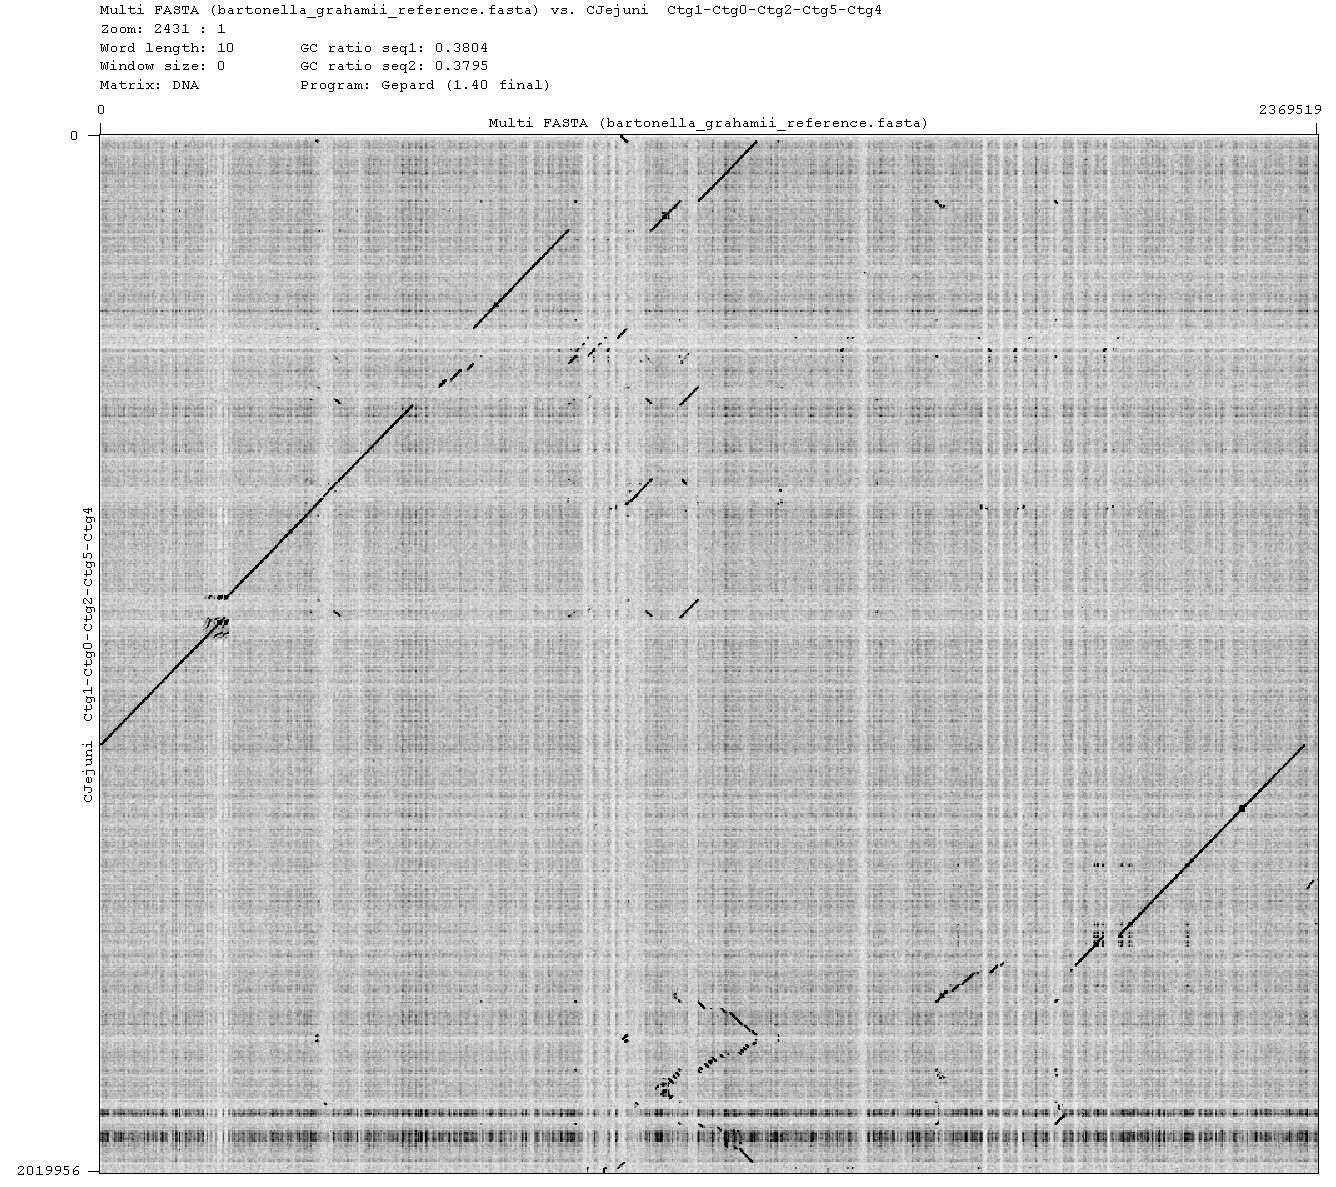
\includegraphics[scale=0.5]{img/graph13.png}
    \caption{BGrahamii - rezultati s Geparda 2}
    \label{fig:bgrahamii2}
\end{figure}

\begin{figure}[H]
    \centering
    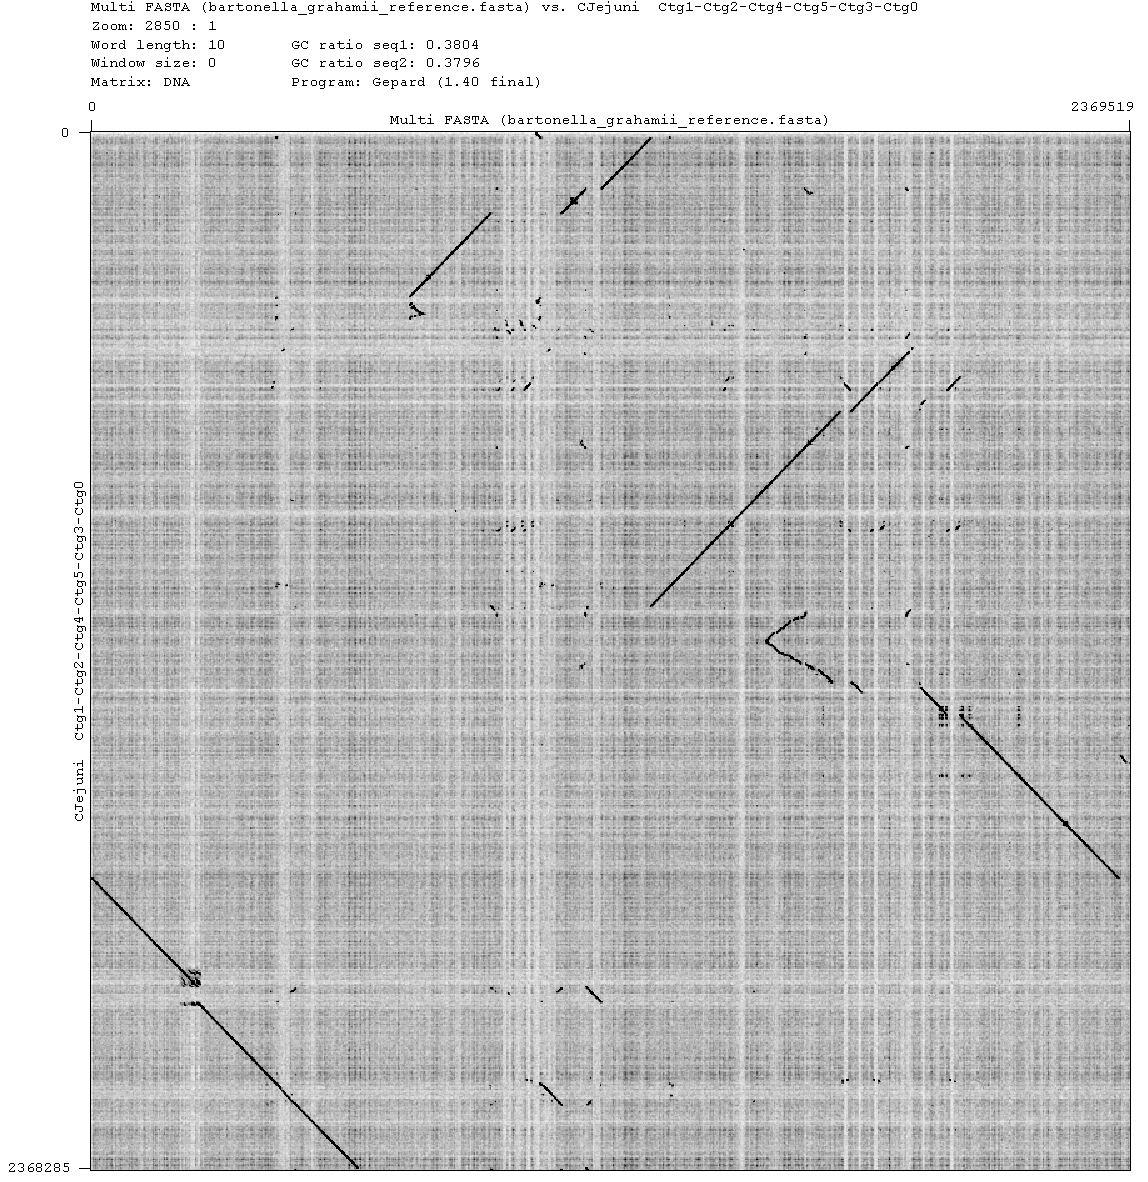
\includegraphics[scale=0.5]{img/graph14.png}
    \caption{BGrahamii - rezultati s Geparda 3}
    \label{fig:bgrahamii3}
\end{figure}